% 图 4.1 分子轨道能级分裂与成键/反键波函数示意
\documentclass[tikz,border=5pt]{standalone}
\usetikzlibrary{arrows.meta}
\usepackage{amsmath}
\usepackage{bm}
\usepackage{fontspec}
\setmainfont{Times New Roman}
\begin{document}
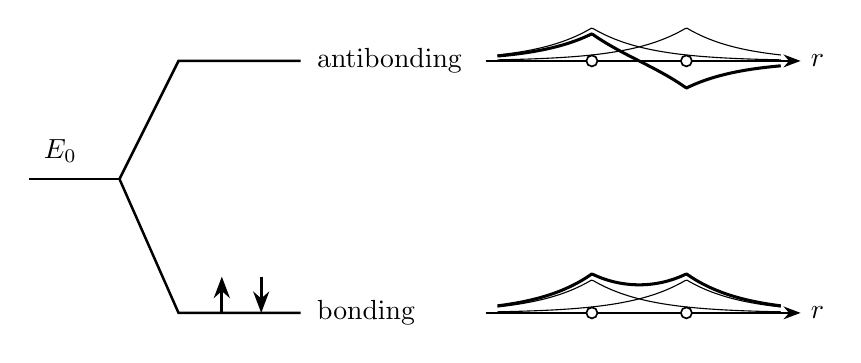
\begin{tikzpicture}[line width=0.8pt,>=Stealth]
% ---------- left: level splitting ----------
\draw[line width=0.9pt] (-0.35,0) -- (0.8,0);
\node[above] at (0.05,0.08) {$E_0$};
\draw[line width=0.9pt] (0.8,0) -- (1.55,1.5) -- (3.1,1.5);
\draw[line width=0.9pt] (0.8,0) -- (1.55,-1.7) -- (3.1,-1.7);
\node[right] at (3.18,1.5) {antibonding};
\node[right] at (3.18,-1.7) {bonding};
% two electrons on bonding level
\draw[line width=1.05pt,->] (2.1,-1.7) -- (2.1,-1.24);
\draw[line width=1.05pt,->] (2.6,-1.24) -- (2.6,-1.7);
% ---------- right: wavefunctions ----------
% antibonding (top)
\draw[->,line width=0.7pt] (5.45,1.5) -- (9.45,1.5) node[right] {$r$};
\draw[line width=0.4pt] plot[domain=5.6:9.2,samples=140]
  (\x,{1.5+0.42*exp(-abs(\x-6.8)/0.7)});
\draw[line width=0.4pt] plot[domain=5.6:9.2,samples=140]
  (\x,{1.5+0.42*exp(-abs(\x-8.0)/0.7)});
\draw[line width=1.1pt] plot[domain=5.6:9.2,samples=200]
  (\x,{1.5+0.42*(exp(-abs(\x-6.8)/0.7)-exp(-abs(\x-8.0)/0.7))});
\draw[fill=white,line width=0.6pt] (6.8,1.5) circle (0.07);
\draw[fill=white,line width=0.6pt] (8.0,1.5) circle (0.07);
% bonding (bottom)
\draw[->,line width=0.7pt] (5.45,-1.7) -- (9.45,-1.7) node[right] {$r$};
\draw[line width=0.4pt] plot[domain=5.6:9.2,samples=140]
  (\x,{-1.7+0.42*exp(-abs(\x-6.8)/0.7)});
\draw[line width=0.4pt] plot[domain=5.6:9.2,samples=140]
  (\x,{-1.7+0.42*exp(-abs(\x-8.0)/0.7)});
\draw[line width=1.1pt] plot[domain=5.6:9.2,samples=200]
  (\x,{-1.7+0.42*(exp(-abs(\x-6.8)/0.7)+exp(-abs(\x-8.0)/0.7))});
\draw[fill=white,line width=0.6pt] (6.8,-1.7) circle (0.07);
\draw[fill=white,line width=0.6pt] (8.0,-1.7) circle (0.07);
\end{tikzpicture}
\end{document}
